% !TEX program = XeLaTeX
% !TEX encoding = UTF-8
\documentclass{article}

\usepackage{xeCJK}
\setCJKmainfont{AozoraMinchoRegular.ttf}
\setCJKsansfont{KodomoRounded-Light.otf}
\setCJKmonofont{KodomoRounded-Light.otf}


%\usepackage{xltxtra}
%\setmainfont[Scale=0.92,BoldFont=IPAPMincho]{IPAPMincho}
%\setsansfont{IPAPGothic}
%\setmonofont{IPAGothic}
%\newfontfamily\engrm[Ligatures=TeX]{IPAPGothic}
%\newfontfamily\engsf[Ligatures=TeX,Scale=0.92]{IPAPGothic}

\XeTeXlinebreaklocale "ja"
\XeTeXlinebreakskip=0pt plus 1pt minus 0.1pt
\XeTeXlinebreakpenalty=0

\XeTeXlinebreaklocale "ja"

\usepackage{url}
\usepackage{cancel}
\usepackage{xspace}
\usepackage{graphicx}
\usepackage{multicol}
\usepackage{multirow}
\usepackage{subfig}
\usepackage{amsmath}
\usepackage{amssymb}
\usepackage[a4paper, width=170mm, top=18mm, bottom=22mm, columnsep=8mm, includeheadfoot]{geometry}
%\usepackage[a4paper, width=140mm, top=18mm, bottom=22mm, includeheadfoot]{geometry}
\usepackage{booktabs}
\usepackage{array}
\usepackage{verbatim}
\usepackage{caption}
\usepackage{natbib}
\usepackage{float}
\usepackage{pdflscape}
\usepackage{mathtools}
\usepackage[usenames, dvipsnames]{xcolor}
\usepackage{afterpage}
\usepackage{pgf}
\usepackage{tikz}
\usepackage{dirtree}
\usepackage[style=american]{csquotes}
\usepackage{amsfonts}
\usepackage{tikz}
\usepackage{tkz-graph}
\usetikzlibrary{arrows,decorations.pathmorphing,automata,positioning,backgrounds,fit,shapes.symbols,chains,intersections}

\newtheorem{definition}{Definition}[section]
\newtheorem{theorem}{Theorem}[section]
\newtheorem{lemma}{Lemma}
\newtheorem{proof}{Proof} [section]



\usepackage[toc, page, title, titletoc, header]{appendix}
\usepackage{marginnote}
\usepackage{tablefootnote}

\renewcommand\appendixname{付\ 録}
\renewcommand\appendixpagename{付\ 録}
\renewcommand\appendixtocname{付\ 録}
\renewcommand\abstractname{要\ 約}


\usepackage{perpage} %the perpage package
\MakePerPage{footnote} %the perpage package command

\usetikzlibrary{shapes.geometric}%
\usepackage{color}
%\usepackage[pages=some, placement=top]{background}
\usepackage{eso-pic}
\usepackage[final]{pdfpages}

%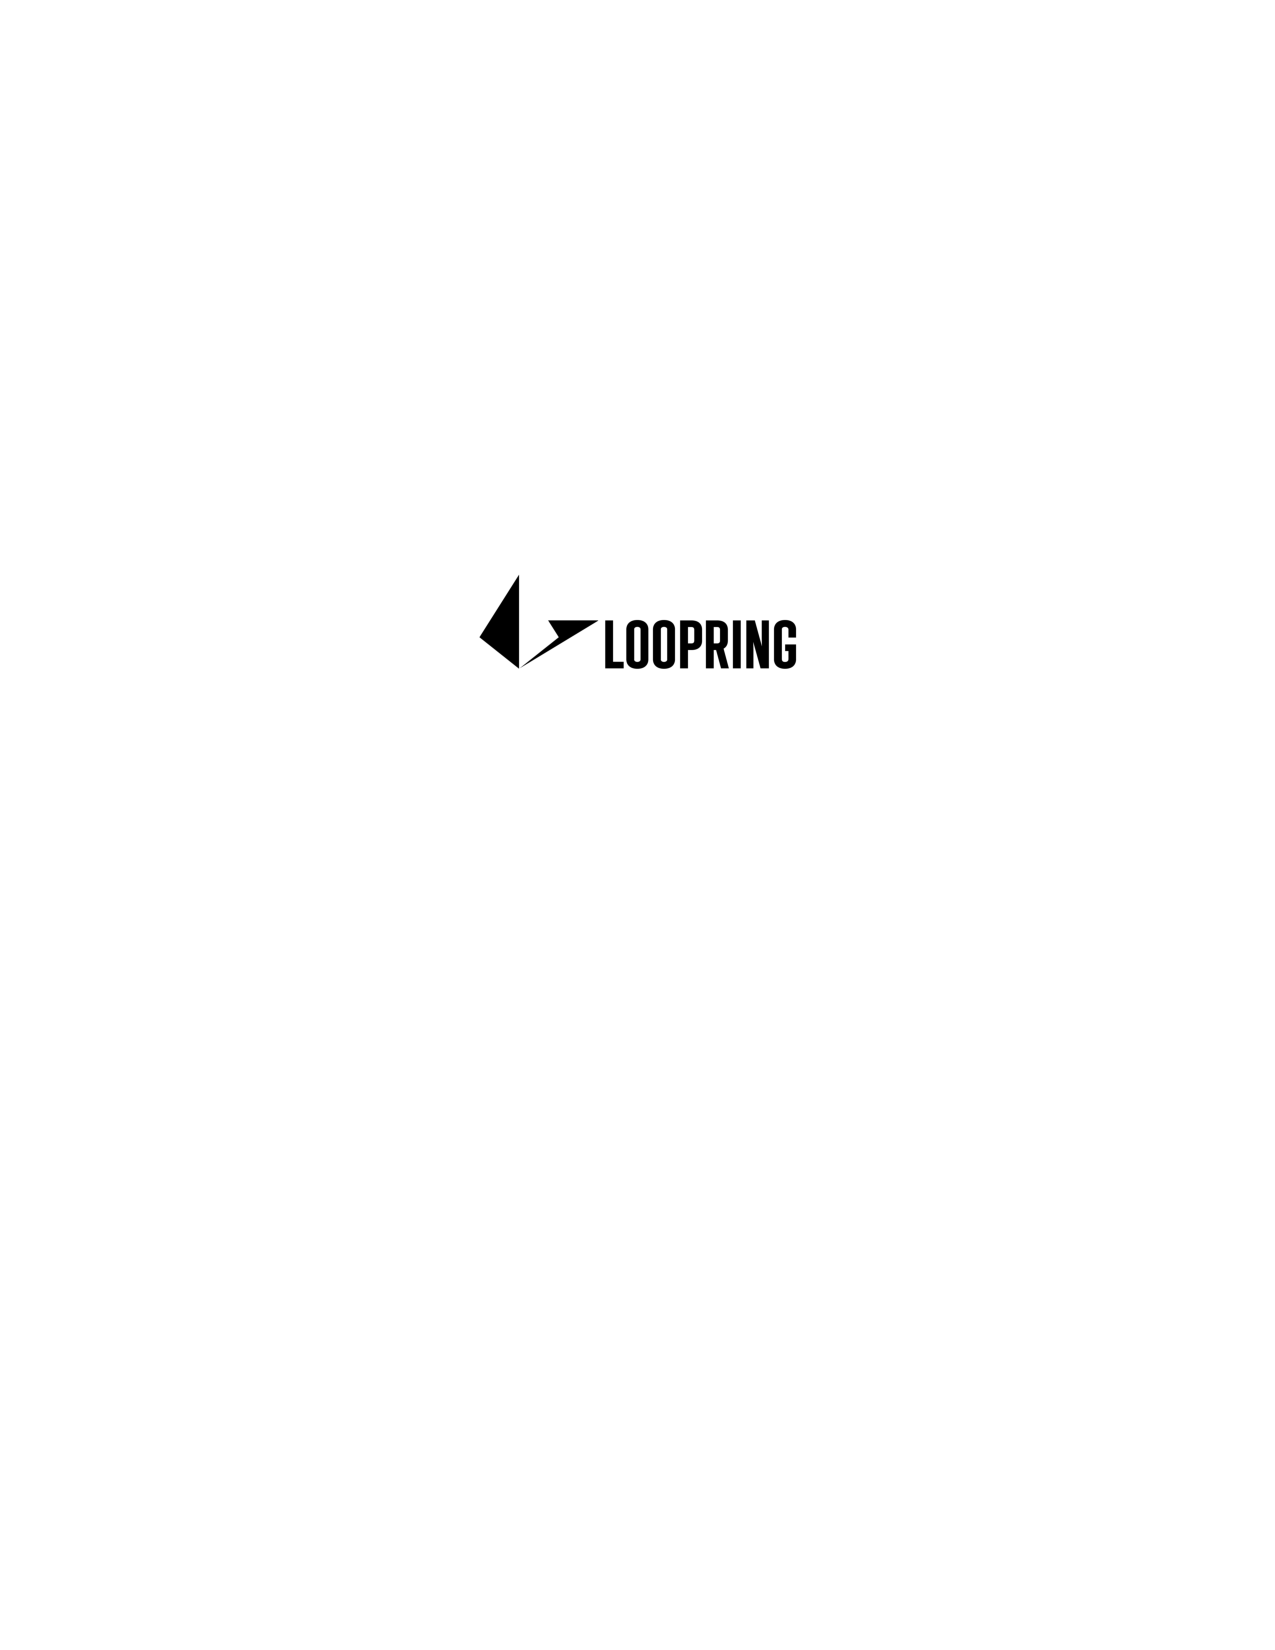
\includepdf[pages=1]{cover}
\hyphenpenalty=750

\title{
{ループリング(LOOPRING):}\\\textbf{分散型トークン取引プロトコル}}
\author{
  Daniel Wang\\
  \texttt{daniel@loopring.org}\\
  \and
  	Jay Zhou\\
  	\texttt{jay@loopring.org}\\
  	\and
  	Alex Wang\\
  	\texttt{alex@loopring.org}\\
  	\and
  	Matthew Finestone\\
  	\texttt{matt.finestone@gmail.com}\\ 
  \\
  \texttt{https://loopring.org}
 }

\makeatletter
\def\CTEX@section@format{\Large\bfseries}
\makeatother

\makeatletter
\newenvironment{tablehere}
 {\def\@captype{table}}
 {}

\newenvironment{figurehere}
 {\def\@captype{figure}}
 {}
\makeatother
%
%\newcommand\BackgroundPic{%
%\put(0, 0){%
%\parbox[b][\paperheight]{\paperwidth}{%
%\vfill
%\centering
%\includegraphics[width=\paperwidth, height=\paperheight, %
%%keepaspectratio]{images/background.jpg}%
%]{images/background.jpg}%
%\vfill
%}}}


%\begin{document}
%\AddToShipoutPicture{\BackgroundPic}
%\maketitle

\begin{document}
%\AddToShipoutPicture{\BackgroundPic}
\maketitle


\begin{abstract}
ループリングは、分散型取引所を構築するためのオープン型プロトコルである。一連の取引・決済機能を持つパブリックスマートコントラクトとして運用し、オフチェーン参加者グループにもオーダー集約・通信できる機能を持つ。ループリングプロトコルは無料且つ拡張可能であり、両替機能を組み込んだ分散型アプリケーション$(dApps)$用の標準化構成要素としても機能する。この相互運用標準は、トラストレス (trustless=信用不要) 匿名取引の実現を促進する。現在の分散型取引プロトコルより最も重要な改良は、オーダー間の整合性 ( ミックスアンドマッチ ) であり、異なる注文オーダーで、2 トークンの取引ペアの制約を取り除くと流動性を大幅に改善する。ほかにも、ループリングは、独自のロバストソリューションを用いて、フロントランニング行為を防ぐ:オリジナルソリューションの提出者より速くブロックにトランザクションを提出しようとする不正行為である。ループリングはブロックチェーンに依存せず、スマートコントラクト機能を備えたブロックチェーンで展開できる。執筆時点では、NEO\cite{atterlonn2018distributed}や、Ethereum \cite{buterin2017ethereum} \cite{wood2014ethereum} や、Qtum \cite{dai2017smart} において動作検証済みである。
\end{abstract}



\begin{multicols}{2}
\section{はじめに\label{sec:introduction}}
ブロックチェーンに基づく資産の増加に伴い、取引相手との資産を交換するニーズも大きく増えた。従来型資産のトークン化を含む数千もの新しいトークンが導入され、ニーズはさらに拡大している。投機的なトークン交換か、交換したユーティリティトークンを介してネットワークへアクセスかにかかわらず、より大きなエコシステムにとって基礎となるのは暗号化資産間での交換能力である。実は、これらの資産に潜在的なエネルギー\cite{desotocapital}が蓄えられている、エネルギーを解放するには、いわゆる資本解錠は、所有権を主張するのみならず、資産の自由譲渡や、変換が必要となる。

そのため、トラストレストークン (対価) の交換は、ブロックチェーン技術において魅力的な実例になる。しかし、現在までも暗号化通貨の愛好家が、殆どのトークン取引を伝統的な集中型取引所で行っていた。従って、ループリングプロトコルが必要とされるのは、ビットコイン\cite{desotocapital}がずっと強調したように、P2P 電子キャシューにとって、「二重支払いを防ぐ為に、信用できるサードパーティー(第三者)が必要とされることは主な利点を失くしている」。同じように、信頼的な、ゲートのあるような中央集権型取引所で取引しなければいけないのは、分散型資産の主な利点を失った。

哲学観点からも、中央集権型取引所における分散型トークンの取引はつじつまが合わない、分散型プロジェクトの理念に反している。中央集権型取引所を利用する際に、多数の実用上のリスクと限界ついては、後ほど詳しく述べる。分散型取引所は$(DEXs)$ \cite{schuh2015bitshares} \cite{bancor} \cite{kyber} これらの問題を対処しようとしている。多くの場合、既存金融機関離れためのブロックチェーン技術を用いて、セキュリティリスクの軽減に成功した。しかし、DEX は新しい経済に重要なインフラストラクチャーになるにつれ、パフォーマンスの改善余地が多大にある。ループリングは、dApp の第三者に非依存的のオープンプロトコルを利用して、インフラストラクチャーためのモジュラー・ツールの提供を目指している。

\section{取引所の現状\label{sec:current_exchange_landscape}}

\subsection{中央集権型取引所の不備}
中央集権型取引所の主なリスクは 3 つ: 1)安全性の欠如、2)透明性の欠如、3)流動性の欠如。

\textbf{安全性の欠如}は、通常、ユーザーがプライベートキー (資金) の管理を1つ集中管理型の実体に委ねることによって生じる。中央集権型取引所にハッカーの不正侵入により、ユーザーが犠牲になる可能性は明らかである。我々は、すべての中央集権型取引所がセキュリティとハッキングのリスクに直面していることについてよく知っているにもかかわらず \cite{coincheckhack}  \cite{mcmillan2014inside} 、トークン取引のための掛け金 (テーブルステークス) として受け入れられている。中央集権型取引所は、引き続きハッカーの「ハニーポット」として攻撃を受けているのは、サーバ上に数百万ドルのユーザー資金を保有しているためである。それに、取引所の開発者も、ユーザーの資金管理に、誠実かつ偶然に誤りを犯すかもしれない。 簡単に言えば、ユーザーは一旦中央集権型取引所に入金したら、自分のトークン管理ができなくなる。

\textbf{透明性の欠如}は、ユーザーに取引所の不正行為による取引リスクをもたらす。ここでは、取引事業者が行った意図的な不正行為を指す。ユーザーは中央集権型取引所で取引しているのが個人の資産より$IOU$である。トークンは一旦取引所ウォレットに送られると、取引所が保管することになり、代わりに一個の$IOU$が提供される。これ以後、ユーザーのすべての取引は、実質的に$IOU$の間である。換金する際、取引所と自分のIOUを清算して、外部ウォレットアドレスにトークンを受け取る。プロセス全体について透明性が欠けており、取引所はシャットダウンしたり、アカウントを凍結したり、倒産などの可能がある。また、ユーザー資産を第三者に貸与するなど、保管しているユーザー資産をその他目的で使用することもあり得る。透明性の欠如は、ユーザーに資金全額がなくなる可能性はないが、取引手数料の増加、ピーク時の需要遅延、規制上のリスク、注文が先行されるなどの犠牲があるかもしれない。

\textbf{流動性の欠如}は、取引事業者から見れば、断片化された流動性は、新しい取引業者の参入を阻害しようとする、2 人の勝者が総取りのシナリオになる。まず、取引ペアが最も多い取引所は勝つ、それはユーザーがすべての取引を1つの取引所でしたがる。その次、オーダーブックが最も大きい取引所は勝つ、それは各トレードペアの好都合な売買スプレッドのためである。このような状況では、初期流動性の構築が難しくなるため、新規参入が困難になる。結果的には、ユーザーから苦情や重大ハッキングがあったにもかかわらず、多くの取引所が高いマーケットシェアを占めている。注意しなければいけないのは、中央集権型取引所は市場シェアが高ければ高いほど、より大きなハッキングの標的になる。

ユーザーから見れば、断片化した流動性はユーザー体験を大幅に低下させる。中央集権型取引所における取引では、ユーザーは取引所自身の流動性プール内で、オーダーブックと、サポートされているトークンペア間でしか取引できないトークン\verb|A|をトークン\verb|B|と交換するには、ユーザーは両方のトークンをサポートする取引所を選ぶか、異なる取引所で登録する、個人情報を開示して。また、売買スプレッドを支払って、BTCまたはETHに対して一旦予備または仲介取引も行う必要がある。結局、ユーザーは、売買スプレッドを支払って、BTC またはETHに対して予備または仲介取引も行わなければならない。最後に、オーダーブックの深さが足りなかったら、品物を減らせなければ取引が完成できない可能性もある。たとえ取引所は自分のプロセス出来高が大きいと称しても、この出来高と流動性が偽りではないとの保証がない\cite{fakevolume}。

その結果、流動性がばらばらになり、エコシステムが断片化され、従来の金融システムのように、わずかの取引所に大量の取引が集中する。グローバルな流動性を持つブロックチェーンには、中央集権型取引所は役に立たない。

\subsection{分散型取引所の欠点}

分散型取引所は中央集権型取引所と一つの違いとは、ユーザーが常にプライベートキー (資産) のコントロールによって、ブロックチェーン基盤で直接に取引する。暗号化通貨のトラストレステクノロジーを活用することで、上記のセキュリティリスクが和らげられる。しかしながら、性能及び構造上の限界に関しては問題が依然として存在する。

流動性がしばしば問題にされるのは、ユーザーは異なる流動性プールと基準を渡って取引相手を探さなければならない。DEXs または dApps が相互運用ための基準を統一しなければ、オーダーはネットワークの広い範囲に渡って共有/伝播されない、断片化した流動性は起こる。板(リミットオーダーブック)の流動性、いわゆる弾力性:確定されたリミットオーダー (指値) どれほど速く再生されるのは、最適取引ストラテジーに著しく影響を及ぼす可能性がある\cite{limitorderliquidity}。このような基準欠如は、流動性の低下につながるのみならず、ユーザーを潜在的に不確かな専有スマートコントラクトに暴露される。

さらに、取引がオンチェーンで行われるため、DEX はブロックチェーン基盤の制約を受け継いでしまう、つまり:スケーラビリティ、実行遅延(マイニング)、オーダー修正に高い費用がつく。結果的には、ブロックチェーンにおけるオーダーブックはうまく調整されず、ブロックチェーンでコード実行はコスト(ガス)がかかる、頻繁に複数の注文取消しは非常に高価になる。

最後に、ブロックチェーンのオーダーブックは一般公開されているため、オーダーを発するトランザクションは、次のブロックでマイニングされ、新しいオーダーブックに置かれるためマイナーに見えるようになっている。このようなリレーはユーザーにフロントランニングリスクと執行価格リスクをもたらす。

\subsection{ハイブリッドソリューション}
上記の理由から、純粋なブロックチェーンベースの取引所には制約があるため、中央集権型取引所と競合できない。オンチェーン固有のトラストレスと中央集権型取引所の取引スピード、オーダー柔軟性の間には妥協点が探せるはずである。ループリングと0x \cite{warren20170x}のようなプロトコルでは、オンチェーン決済のソリューションを拡張して、オフチェーンのオーダー管理と結合する。これらのソリューションは、オープン型スマートコントラクトを中心に展開され、複数の関数をオフチェーンで実行することによって、ノードに柔軟性を与え、ネットワークに重要な役割を果たせて、スケーラビリティの限界を突き止めたいが、ハイブリッドモデルにも同じく欠点が残っている\cite{costofdecent}。 この論文を通じて、ループリングプロトコルは、ハイブリッドソリューションに関する建設的な意見を提案する。

\section{ループリングプロトコル\label{sec:loopring_protocol}}
ループリング自体は DEX ではない、複数のブロックチェーンに渡って、DEX を構築するプロトコルモジュールである。我々は従来の取引所の構成要素を分解し、パブリックスマートコントラクトと分散型参加者に代替させる。ネットワークでの役割は、ウォレット、リレー、流動性シェアリング・ブロックチェーン・コンソーシアム、オーダーブックブラウザ、リングマイナー、資産トークン化サービスを含む。それぞれの参加者を定義する前に、まずループリングオーダーを知る必要がある。

\subsection{オーダーリング\label{sec:order_ring}}
我々はループリングオーダーを単一指向性オーダーモデル「UDOM」\cite{coinport2014udom}で表す。ビットとアスクの代わりに、 UDOM はオーダーをトークン取引リクエスト「$amountS/amountB$」(売/買数量)と表す。オーダーは単なる 2つトークンの間での交換レードになる、ループリングプロトコルの強い特徴は環状トレードにおけるマルチオーダーのミックスとマッチングである。 1つ取引ペアの代わりに、16 個までのオーダーを利用し、流動性の大幅な向上および潜在的な価格改善が期待されている。

\begin{center}
\begin{figurehere}
\centering
\tikzstyle{block} = [draw, fill=blue!20, rectangle, 
    minimum height=3em, minimum width=6em]
\tikzstyle{sum} = [draw, fill=blue!20, circle, node distance=1cm]
\tikzstyle{input} = [coordinate]
\tikzstyle{output} = [coordinate]
\tikzstyle{pinstyle} = [pin edge={to-,thin,black}]

\begin{tikzpicture}[
    auto, 
    node distance=2cm,
    >=latex',
    font=\normalfont,
    order/.style={
		scale=0.8,
		rectangle,
		rounded corners,
		draw=black, 
		text centered,
%		text width=10cm,
		minimum height=17mm,
		fill=white
	},
	label/.style={
		scale=0.8
	}
  ]
    % We start by placing the blocks

  \node [order] (order2) 
 {%
 \begin{tabular}{l}
  \textbf{オーダー\#2}\\
  \textbf{所有者:Y}\\
  \textbf{売り数量:9B}\\
  \textbf{買い数量:12C}
 \end{tabular}
 };
 
  \node [order, below of=order2, xshift=-3.5cm] (order1) 
 {%
 \begin{tabular}{l}
  \textbf{オーダー\#1}\\
  \textbf{所有者:X}\\
  \textbf{売り数量:10000A}\\
  \textbf{買い数量:2B}
 \end{tabular}
 };
 
 
  \node [order, below of=order2, xshift=3.5cm] (order3) 
 {%
 \begin{tabular}{l}
  \textbf{オーダー\#3}\\
  \textbf{所有者:Z}\\
  \textbf{売り数量:100C}\\
  \textbf{買い数量:160A}
 \end{tabular}
 };
 
 \draw [draw,->] (order1) -- node [label] {\textbf{7898A}} (order3);
 \draw [draw,->] (order2) -| node [label, xshift=-1.8cm] {\textbf{8B}} (order1);
 \draw [draw,->] (order3) |- node [label, xshift=1cm, yshift=0.24cm] {\textbf{98C}} (order2);

\end{tikzpicture}

\caption{3つのオーダーでのオーダー・リング}
\label{fig:ring}
\end{figurehere}
\end{center}

上の図は3つオーダーで組み合わせたオーダーリングを示している。各オーダーの売りたいトークン(\verb|tokenS|)は、ほかのオーダーの買いたいトークン (\verb|tokenB|)になっている。各オーダーに反対オーダーを建つ必要とせず、欲しいトークンに交換できるループが生まれる。このようなオーダーリングにおいて、一般的な取引ペアも当然取引できるが、本質的にはオーダーリングのスペシャルケースである。


\begin{definition}[オーダーリング]$C_{0}$, $C_{1}$, $\cdots$, $C_{n-1}$ は$n$個の異なる種類のトークンとし、 $O_{0\rightarrow 1}$, $\cdots$, $O_{i\rightarrow i\oplus 1}$, $\cdots$, $O_{n-1 \rightarrow 0}$ は$n$個の注文とする。これらの注文は一つのオーダーリングを形成する:
$$O_{0\rightarrow 1} \rightarrow \cdots \rightarrow O_{i\rightarrow i\oplus 1} \rightarrow \cdots \rightarrow O_{n-1\rightarrow 0} \text{, }$$
nはオーダーリングの長さである場合、 $i\oplus 1 \equiv i+1 \mod n$ となる。
\end{definition}

全構成要素のトランザクションが、ユーザーが暗黙に指定したオリジナルの交換レートと等しいか、より良いレートで執行されるとオーダーリングは有効になる。その有効性を検証するには、ループリングプロトコルのスマートコントラクトがリングマイナーからオーダーリングを受け取らなければならない、それに、オーダーのオリジナル交換レートの積は1 以上になる必要だ。

アリスとボブがトークン \verb|A| と \verb|B| を取引したいと仮定してみよう。アリスはトークン \verb|A| を15個所有し、それを使ってトークン \verb|B| を 4 個に取替えしたい。 ボブはトークン \verb|B| を 10 個所有しトークン \verb|A| を 30 個にしたい。

買い手と売り手はそれぞれ誰でしょうか?我々がどっちの資産を参照価格に想定しようによる。例えば、トークン \verb|A| が参照価格にされた場合、アリスはトークン \verb|B|を値段 $\displaystyle \frac{15}{4}=3.75A$ で購入した、ボブは $\displaystyle \frac{30}{10} = 3.00A$ の値段でトークン \verb|B| を10個販売した。トークン \verb|B| を参考価格に想定する場合、アリスは$\displaystyle \frac{4}{15} = 0.26666667B$の値段で 15 個のトークン \verb|A| を販売し、ボブは$\displaystyle \frac{10}{30} = 0.33333334B$ の値段で 10 個のトークン \verb|A| を購入したい。よって、だれが買い手や売り手は勝手だ。

1 番目のケースには、アリスはボブが自分のトークンに付けた売り価格 ($3.00$\verb|A|)より高い価格の ($3.75$\verb|A|)を支払いたい、2 番目のケースでは、ボブはアリスが自分トークンに付けた売り価格 ($0.26666667$\verb|B|)より高い価格 ($0.33333334$\verb|B|)を支払いたい。買い手は売り手が付けた値段以上を支払う意思があるならば、取引はいつでも可能のが明白だ。

\begin{equation}
{{15\over 4} \over {30\over 10}} = {{10\over 30} \over {4\over 15}}={15 \over 4} \cdot {10 \over 30} = 1.25 > 1
\end{equation}
  
したがって、$n$個注文集合の全部あるいは一部を満たすには、それぞれ買い注文の交換レートの積は 1 以上かどうかを知る必要がある。そうであれば、注文$n$の一部或いは全部は満たされる\cite{supersymmetry}。

さらに第三相手のチャーリーが登場すると、アリスがトークン\verb|A|の $x_{1}$ をトークン\verb|B|の $y_{1}$ に、ボブはトークン\verb|B| の $x_{2}$ をトークン \verb|C|の $y_{2}$ に、そして、チャーリーはトークン \verb|C| の $x_{3}$ を、トークン\verb|A|の $y_{3}$ に、それぞれを取替えたい。

必要なトークンはそろっていれば、次の式を満たせば取引は可能になる:

\begin{equation}
{{x_1 \cdot x_2 \cdot x_3 \over y_1 \cdot y_2 \cdot y_3} \geq 1}
\end{equation}

ループリングオーダーの詳細について、\ref{anatomy} で後述する。


\section{エコシステムの参加者\label{sec:ecosystem}}
次のエコシステムの参加者は、中央集権型取引所が提供すべき全機能を共同で提供する。

\begin{itemize}

\item \textbf{ウォレット}:普通のウォレットサービス或いはインターフェイスは、ユーザーにトークンへのアクセスとループリングネットワークへのオーダー送信を提供する。ウォレットはリングマイナーと手数料をシェアリングすることによって、オーダー生成に意欲を発揮する(詳細は \ref{sec:token}を参照)。 将来の取引がユーザー個人のウォレット内で安全に行われると信じ、プロトコルを通じて、これらの流動性 (資金) プールを結びつけるのが最も重要である。

\item \textbf{流動性シェアリング・ブロックチェーン・コンソーシアム/リレーメッシュ}:オーダーと流動性シェアリングためのリレーメッシュネットワークである。ノードがループリング リレーソフトウェアを実行すると、既存のネットワークに接続できる、コンソーシアムブロックチェーンを介して他のリレーと流動性をシェアリングできる。我々は構築している最初のコンソーシアムブロックチェーンでは、リアルタイム(1-2秒ブロック)でオーダーシェアリングできるし、新たなノードでより速いダウンロードのために旧い履歴を削除する。とりわけ、リレーはコンソーシアムに参加する必要がない、彼らは単独で動けるし、他者と流動性をシェアリングしないし、或いは自身の流動性シェアリングネットワークをはじめ、管理する。

\item \textbf{リングマイナー}::リレーは、ウォレットやリレーメッシュからオーダーを受け取り、パブリックオーダーブックと取引履歴を維持し、任意でその他リレー(任意のオフチェーン媒体を介して)および/或いはリレーメッシュにオーダーを伝送するノードである。リングマイニングはリレーの特徴であって、要件ではない、 計算が重く、完全にオフチェーンで行われる。 我々はリングマイニング機能を持つリレーを「リングマイナー」(\enquote{Ring-Miners})と呼ぶ、異なるオーダーをつなげ、オーダーリングを生成する。リレーは以下の三つにおいて自由である (1)その他リレーとコミュニケーションの取る方法、(2)オーダーブックの構築する方法、(3)オーダーリング(マイニングアルゴリズム)のマイニング方法。

\item \textbf{ループリングプロトコル・スマートコントラクト(LPSC)}:
公開且つ無料のスマートコントラクトのセットである、リングマイナーから受信したオーダーリングを検査し、ユーザーのためにトークンをトラストレス的に処理・転送し、リングマイナーとウォレットに手数料を割り当て、イベントを起す。 リレー/オーダーブラウザは、これらのイベントに監視し、オーダーブックと取引履歴を最新の状態に保つ。 詳細については、付録 \ref{app:protocol_ethereum}を参照してください。

\item \textbf{資産トークン化サービス(ATS)}:ループリングで直接に取引できない資産間のブリッジである、 信頼できる企業や組織に運営されている中央集権型サービスである。 ユーザーは、資産(実物、法定通貨、その他チェーンのトークン)を預託し、トークンを発行し、将来これらを預金に引き換えられる。 ループリングは(適切な解決策が存在するまで)クロスチェンで取引プロトコルではないが、ATS は ERC20 トークンを実物資産やその他のロックチェーンの資産と取引出来るように \cite{ERC20} する。

\end{itemize}

\section{交換プロセス\label{sec:process}}

\begin{enumerate} 

\item \textbf{プロトコル認証}:図\ref{fig:process} にように、トークンを交換したいユーザー\verb|Y|は、売りたいトークン\verb|B|(\verb|amountS|)の取り扱いを LPSC に認可し、処理できるように。これより、ユーザーのトークンはロックされず、オーダーがプロセス中にも自由に移動できる。

\item \textbf{オーダー生成}:トークン\verb|B|vs トークン\verb|C|の成り行きレートとオーダーブック(板)は、リレーやオーダーブックブラウザのようなその他ネットワーク接続仲介経由で提供された。 ユーザー\verb|Y|は、任意の統合ウォレット・インターフェースを介して、\verb|amountS|、\verb|amountB| とその他パラメータを明記した上オーダー(指値オーダー)を発注する。一定数量の LRx が、リングマイナーの手数料として、オーダーに加えられる。 LRx 料金は、高ければ、高いほどリングマイナーにより早く処理される。 オーダーハッシュにはユーザー\verb|Y|のプライベートキーで署名される。

\item \textbf{オーダーブロードキャスト}:ウォレットはオーダーとその署名を 1 つまたは複数のリレーに送信してから、 リレーはパブリックオーダーブックを更新する。 このプロトコルでは、先着順などで特定方法で、オーダーブックを作成するように要求しない。それより、リレーはオーダーブックを作成する際に自由裁量の余地を持つ。

\item \textbf{流動性シェアリング}:リレーは任意の通信媒体を経由して他のリレーにオーダーをブロードキャストする。 また、ノード間はどのように相互作用や、相互作用するかどうかは柔軟性がある。安定しているネットワーク接続を促進するために、ブロックチェーンコンソーシアムに流動性シェアリングリレーメッシュを作り上げた。前のセクションで述べたように、このリレーメッシュは速度と包括性のため最適化されている。

\begin{center}
\begin{figurehere}
\centering
\tikzstyle{block} = [draw, fill=blue!20, rectangle, 
    minimum height=3em, minimum width=6em]
\tikzstyle{sum} = [draw, fill=blue!20, circle, node distance=1cm]
\tikzstyle{input} = [coordinate]
\tikzstyle{output} = [coordinate]
\tikzstyle{pinstyle} = [pin edge={to-,thin,black}]

\begin{tikzpicture}[
    auto, 
    scale=0.6,
    node distance=2.5cm,
    >=latex',
    font=\normalfont,
    order/.style={
		rectangle,
		scale=0.6,
		rounded corners,
		draw=black, 
		text centered,
%		text width=5cm,
		minimum height=12mm,
		minimum width=30mm,
		fill=white
	},
	role/.style={
		circle,
		scale=0.6,
		draw=black, 
		text centered,
%		text width=5cm,
		minimum height=12mm,
		minimum width=12mm,
		fill=white
	},
	steps/.style={
		circle,
		scale=0.6,
		draw=black, 
		text centered,
%		text width=5cm,
%		minimum height=12mm,
%		minimum width=12mm,
		fill=black,
		text=white
	},
	account/.style={
		circle,
		scale=0.6,
		draw=black, 
		text centered,
%		text width=5cm,
		minimum height=16mm,
		minimum width=16mm,
		fill=white
	},
	label/.style={
	  scale=0.6
    }
  ]

 
 \node [role] (user1)  {ユーザーX};
 \node [role, below of=user1] (user2)  {ユーザーY};
 \node [role, below of=user2] (user3)  {ユーザーZ};
 \node [role, below of=user3, fill=gray!20] (relay1)  {リレーM};
 \node [role, below of=relay1, fill=gray!20] (relay2)  {リレーN};

 
 \node [order, left of=user1, xshift=-1cm] (order1) 
 {%
 \begin{tabular}{l}
  \textbf{オーダー 1}\\
  \textbf{所有者:X}\\
  \textbf{売り数量:10000A}\\
  \textbf{買い数量:2B}
 \end{tabular}
 };
 
 \draw [draw, ->]  (user1) -- (order1) [label]{};
 \draw [bend right,->] (order1) to node [auto, scale=0.7] {} (relay1);
 \draw [bend right,->] (order1) to node [auto, scale=0.7] {} (relay2);
% \draw [draw, ->]  (order1) |- (relay1) [label]{};
% \draw [draw, ->]  (order1) |- (relay2) [label]{};
 
 \node [order,left of=user2, xshift=-1.5cm] (order2) 
 {%
 \begin{tabular}{l}
  \textbf{オーダー 2}\\
  \textbf{所有者:Y}\\
  \textbf{売り数量:9B}\\
  \textbf{買い数量:12C}
 \end{tabular}
 };
 \draw [draw, ->]  (user2) -- (order2) [label]{};
 \draw [bend right,->] (order2) to node [auto, scale=0.7] {} (relay1);
 \draw [bend right,->] (order2) to node [auto, scale=0.7] {} (relay2);
% \draw [draw, ->]  (order2) |- (relay1) [label]{};
% \draw [draw, ->]  (order2) |- (relay2) [label]{};
% 
\node [order, left of=user3, xshift=-2cm] (order3) 
 {%
 \begin{tabular}{l}
  \textbf{オーダー 3}\\
  \textbf{所有者:Z}\\
  \textbf{売り数量:100C}\\
  \textbf{買い数量:160A}
 \end{tabular}
 };
 \draw [draw, ->]  (user3) -- (order3) [label]{};
 \draw [bend right,->] (order3) to node [auto, scale=0.7] {} (relay1);
 \draw [bend right,->] (order3) to node [auto, scale=0.7] {} (relay2);
% \draw [draw, ->]  (order3) |- (relay1) [label]{};
% \draw [draw, ->]  (order3) |- (relay2) [label]{};
 
% // The Ring
\node [order, 
yshift=-2.75cm,
xshift=-2.75cm,
below of=relay2,
fill=gray!10,
minimum width=4.5cm,
minimum height=7cm] (ring) {};


\node [order, dashed, below of=relay2,yshift=-0.7cm,xshift=-2.5cm] (order11) 
 {%
 \begin{tabular}{l}
  \textbf{オーダー 1}\\
  \textbf{所有者:X}\\
  \textbf{売り数量:10000A}\\
  \textbf{買い数量:2B}
 \end{tabular}
 };
 \node [order, dashed,below of=order11,xshift=-0.25cm,yshift=0.7cm] (order21) 
 {%
 \begin{tabular}{l}
  \textbf{オーダー 2}\\
  \textbf{所有者:Y}\\
  \textbf{売り数量:9B}\\
  \textbf{買い数量:12C}
 \end{tabular}
 };
\node [order, dashed,below of=order21,xshift=-0.25cm,yshift=0.7cm] (order31) 
 {%
 \begin{tabular}{l}
  \textbf{オーダー 3}\\
  \textbf{所有者:Z}\\
  \textbf{売り数量:100C}\\
  \textbf{買い数量:160A}
 \end{tabular}
 };
 
 % // The blockchain
\node [
rectangle,
fill=gray!20, 
right of=user1,
yshift=-5cm,
xshift=0.1cm,
scale=0.7,
minimum width=3.2cm,
minimum height=17cm] (ブロックチェーン) {\parbox[b][15cm]{1.3cm}{ブロックチェーン}};
% blockchain accounts
  \node [account, right of=user1, xshift=1cm] (account1)  {アカウントX};
  \node [account, right of=user2, xshift=1cm] (account2)  {アカウントY};
  \node [account, right of=user3, xshift=1cm] (account3)  {アカウントZ};
  \node [account, right of=relay1, xshift=1cm] (account4)  {アカウントM};
  \node [account, right of=relay2, xshift=1cm] (account5)  {アカウントN};
  \node [account, double, below of=account5, yshift=-1.4cm] (psc)  {LPSC};
  
 \draw [draw, ->]  (user1) -- (account1) [label]{};
 \draw [draw, ->]  (user2) -- (account2) [label]{};
 \draw [draw, ->]  (user3) -- (account3) [label]{};
% \draw [draw, ->]  (relay1) -- (account4) [label]{};
% \draw [draw, ->]  (relay2) -- (account5) [label]{};
 \draw [draw, double, thick]  (relay1) to node [auto, scale=0.6, xshift=0.5cm, yshift=0.3cm] {流動性シェアリング}  (relay2) [label]{};
% \draw [draw, ->]  (relay1) -- (ring) [label]{};
 \draw [draw, ->]  (relay2) to node [auto, scale=0.6, xshift=-5cm, yshift=0.5cm] {リングマイニング}  (ring) [label]{};
 \draw [draw, ->]  (ring) to node [auto, scale=0.6, xshift=1.5cm,  yshift=0.5cm] {リングサブミット} (psc) [label]{};
 
 \draw [bend left,->] (account1) to node [auto, scale=0.7] {\textbf{7898 A}} (account3);
 \draw [bend left,->] (account2) to node [auto, scale=0.7] {\textbf{8 B}} (account1);
 \draw [bend left,->] (account3) to node [auto, scale=0.7] {\textbf{98 C}} (account2);
 
 \draw [bend left,->, dashed] (account1) to node [auto, scale=0.7] {} (account5);
 \draw [bend left,->, dashed] (account2) to node [auto, scale=0.7] {} (account5);
 \draw [bend left,->, dashed] (account3) to node [auto, scale=0.7, xshift=.5cm] {\textbf{手数料}} (account5);
  
  
% \draw [draw,->] (order1) -- node [label] {\textbf{7898 A}} (order3);
% \draw [draw,->] (order2) -| node [label, xshift=-1.8cm] {\textbf{8 B}} (order1);
% \draw [draw,->] (order3) |- node [label, xshift=1cm, yshift=0.24cm] {\textbf{98 C}} (order2);

\node [steps, right of=user2, xshift=-0.6cm] () {1};
\node [steps, left of=user2, xshift=0.8cm] () {2};
\node [steps, left of=relay2, xshift=0.3cm, yshift=1cm] () {3};
\node [steps, left of=relay1, xshift=3.6cm, yshift=-1.6cm] () {4};
\node [steps, below of=relay2, xshift=0.3cm, yshift=1cm] () {5};
\node [steps, right of=account3, xshift=-0.6cm] (step5) {6};

 \draw [bend right, ->]  (psc) to node [auto, scale=0.7, xshift=0.5cm] {決済} (step5) [label]{};
 
\end{tikzpicture}

\caption{ループリング取引プロセス}
\label{fig:process}
\end{figurehere}
\end{center}


\item \textbf{リングマイニング(オーダーマッチング)}:リングマイナーは、オーダーをその他多数のオーダーをマッチングすることによって、指定されたまたはそれ以上の交換レートで、オーダーの全部または一部を満たせようとする。リングマイニングこそ、プロトコルがあらゆるペアに高い流動性を提供できる訳である。もし実行レートがユーザー\verb|Y|の指定より良いであれば、マージンはオーダーリング内に全オーダーでシェアリングされる。報酬として、リングマイナーは、マージンの一部(マージン・スピリット、LRx をユーザーに返す)を請求するか、または単にLRx料金を保留する。

\item \textbf{検証と決済}:LPSC がオーダーリングを受信し、複数チェックを行う、 リングマイナーから受け取ったデータを検証するためである。それに、オーダーリングが完全にまたは部分的に決済されるかどうかを決める(リング内オーダーの充足率とユーザーウォレット内のトークン残高による)。全てのチェックが合格であれば、コントラクト (LPSC) は自動的にトークンをユーザーに譲渡すると同時に、リングマイナーとウォレット料金の支払いを行う。もし LPSC はユーザー \verb|Y| が残高不足と判明した場合は、縮尺が実施される;仮に十分な資金がアドレスに入金されたら、縮小されたオーダーは自動的に元サイズまで拡大される、キャンセルと違うのは、取り消しはリバース不可の片方向マニュアル操作である。

\end{enumerate}





%
%\end{multicols}
%
%\begin{center}
%\begin{figurehere}
%\includegraphics[height=8cm]{images/en_protocol.png}
%\caption{Loopring Trading Process}
%\label{fig: Loopringrotocol}
%\end{figurehere}
%\end{center}
%
%\begin{multicols}{2}


\section{運用上の柔軟性\label{sec:business_model}}

注意しなければならないのは、ループリングのオーペン基準は参加者に非常に大きな操作柔軟性を与える。 参加者は、新たなビジネスモデルを無料で実装できるし、ユーザーに価値を提供すると同時にプロセスの出来高やその他基準によx料金を稼げる (選択した場合)。 エコシステムはモジュール化されており、より多くのアプリケーションの参加をサポートする。

\subsection{オーダーブック\label{sec:order_book}}
リレーがオーダーブックを設計する際、好きな方法でユーザーオーダーを表示し、マッチングできる。最初に実装した独自のオーダーブックは OTC モデルで、価格のみに基づいて配置される。つまり、オーダーのタイムスタンプは、オーダーブックとは無関係だ。しかし、リレーは自分のオーダーブックを自由に設計できる、典型的な中央集権型取引のマッチングエンジンのように、タイムスタンプを重視しながら注文値段でランク付ける。リレーがこの種のオーダーブックを提供する傾向になったら、ウォレットを所有/統合して、オーダーをただ1つのリレーのみに送信する。そうなると、このリレーが時間順にオーダーをマッチングできる。 このような構成は可能となる。

一方、ほかの DEX プロトコルでは、リレーに一定のリソースを要求する:買いオーダー発注用の初期トークン残高が求められる、その一方、ループリングリレーでは、取引成立にマッチング可能なオーダーを見つければ、初期トークンがなくても可能である。

\subsection{流動性のシェアリング\label{sec:liquidity_sharing}}
リレーは、互いにどのように流動性(オーダー)をシェアリングするのが自由に設計できる。 我々のブロックチェーンコンソーシアムは、流動性シェアリングをやり解ける為の一つの解決策に過ぎず、エコシステムは好きなように、自由にコミュニケーションする。 ブロックチェーンコンソーシアムに参加するほかに、自身の流動性シェアリングを構築して、管理する、自分に相応しいルールやインセンティブを決める。前述のように時間順にオーダー実行のウォレットのように、リレーは単独で動作することもできる。もちろん、ネットワーク効率を求めるために、他のリレーと通信するのは、明らかに有利であるが、異なるビジネスモデルは独自のシェアリングデザインもを評価し、多様な方法で手数料分割する。

\section{プロトコルの仕様\label{sec:protocol}}

\subsection{オーダーの解析\label{anatomy}}
オーダーというのは、ユーザーの取引の意図を表すデータの群れである。ループリングにおけるオーダーは、片方向オーダーモデル(the Uni-Directional Order Model)
あるいは UDOM で次のように定義されている。

\begin{verbatim}
message Order { 
 address protocol;
 address owner;
 address tokenS;
 address tokenB;
 uint256 amountS;
 uint256 amountB;
 unit256 lrcFee
 unit256 validSince; // システム時間
 unit256 validUntil; // システム時間
 uint8 marginSplitPercentage; // [1-100]
 bool buyNoMoreThanAmountB;
 uint256 walletId; // デュアル認証アドレス
 address authAddr; // v, r, s は署名のパーツ
 uint8 v;
 bytes32 r;
 bytes32 s;      
 // 中ある認証プライベートキー
 // オーダーハッシュ値計算に使わない,
 // よって署名されてない.
 string authKey;
} 
\end{verbatim}


オーダーの発信元を確認するため、ユーザーのプライベートキーでパラメータのハッシュ値に対して署名する \verb|authAddr| を除く。\verb|authAddr| パラメータは、オーダーの一部であるオーダーリングに署名するために使われており、フロントランニングを防ぐために。 詳細は \ref{sec:dual_authoring}を参照してください。フィールド \verb|v|、\verb|r|、と \verb|s| は署名を表している、オーダーパラメータと共にネットワーク上に送信される。存続期間にオーダーは変更されないことが保証される。 オーダーは決して変更されないが、プロトコルは他の変数やアドレス残高に基づいて現在の状態を算出する。

UDOM には価格(本来であれば浮動小数点数でなければならない)が含まれていないが、代わりにレート(\verb|rate|)や $r$ を使って、\verb|amountS|/\verb|amountB|をあらわす。 レートは浮動小数点数ではなく、式であり、必要に応じて他の符号なし整数で計算し、すべての中間結果を符号なし整数として維持し、計算精度を向上させる。

\subsubsection{買い数量}
リングマイナーがオーダーをリングマッチする時、より良いレートで実行される可能性があり、ユーザーが指定した買い数量 (\verb|amountB|) より多いトークン \verb|tokenB| を得られる。しかし、もし \verb|buyNoMoreThanAmountB| が \verb|True| に設定すると、ループリングプロトコルがユーザーにトークン \verb|tokenB| を \verb|amountB| 以上の受け取らないようにする。 したがって、UDOMの \verb|buyNoMoreThantokenB| パラメータは、全オーダーが満たされる時期を決める。 \verb|buyNoMoreThantokenB| は、売り数量 (\verb|amountS|) または買い数量 (\verb|amountB|)のいずれかに上限に適用し、ユーザーが従来の売買オーダーよりも細かく取引意向を設定できる。

たとえば、\verb|amountS| = 10で、\verb|amountB| = 2 の場合、取引レート $r$ = 10/2 = 5となる。したがって、ユーザーは1つのトークン \verb|B| に、5 つのトークン \verb|S| を売りたい。リングマイナーは、ユーザーにレート 4 を見つけた、つまりユーザーはトークン \verb|B| を、2 ではなく 2.5 を受け取れる。
しかし、ユーザーがトークン \verb|B| を 2 つしかほしくない場合は、 \verb|buyNoMoreThanAmountB| のフラグを \verb|True| に設定すれば、LPSC は取引を倍率レート 4 で実行し、ユーザーにはトークン \verb|B| ごとに、4 つのトークン \verb|tokenS| を売る、つまりトークン \verb|tokenS| を 2 つ節約できた。注意してほしいのは、これらにはマイニング手数料は考慮されていない(詳細は \ref{sec:fee_model} を参照)。

実際、我々はオーダーを簡略化された形式でも表現できる。

\begin{verbatim}
	      Order(amountS,tokenS,
	            amountB,tokenB,
	            buyNoMoreThantokenB)
\end{verbatim}

従来の取引所の ETH / USD マーケットには、一般な売買モデルでは、下記 1 番と 3 番でオーダーを表現できるが、その他 2つオーダーはできない。

\begin{enumerate}
\item 価格 300 USD/ETH で10 ETHを売る。 このオーダーは、 \verb|Order(10, ETH, 3000, USD, False)| で表す。
\item 価格 300 USD/ETH で10 ETHを売って、3000 USD を入手する。 このオーダーは次のように表現できる: \verb|Order(10, ETH, 3000, USD, True)| 。
\item 価格 300 USD/ETH で10 ETHを買い。このオーダーは、 \verb|Order(3000, USD, 10, ETH, True)|で表す。
\item 3000米ドルを費やし、価格 300 USD/ETHでできるだけ多くのETHを買う。この注文は、\verb|Order(3000, USD, 10, ETH, False)| で表す。
\end{enumerate}


\subsection{リングの検証\label{sec:ring_verification}}
ループリングスマートコントラクトは交換レートや取引数量に関するの計算をしないが、リングマイナーから提供されたこれらの値を受け取って、検証しなければならない。 計算は、リングマイナーに実行される理由は主に以下の 2つ:
(1) スマートコントラクトのプログラミング言語は、例えば、Ethereum 上の solidity \cite{dannen2017introducing}、浮動小数点数演算をサポートしていない、特に $pow(x、1 / n )$ (浮動小数点数のn乗根を計算する)。 (2) ブロックチェーン上の計算とコストを減らすため、計算プロセスはオフチェーンにするのが望ましい。


\subsubsection{サブリングの検証 \label{sec:sub_ring_check}}
このステップは、アービトレィジャーがオーダーリング内で新規注文の実行による利益の不正取得。本来では、一旦リングマイナーが有効なオーダーリングを見つけると、オーダーリングに他のオーダーを追加してユーザーのマージン(取引倍率の割引)を全部奪おうとなる。以下図 \ref{fig:subring} に示しているように、$x1$, $y1$, $x2$, $y2$を慎重に計算し、全オーダーレートの積をピッタリ 1 にすれば、レート割引がない。

\begin{center}
\begin{figurehere}
\centering
\tikzstyle{block} = [draw, fill=blue!20, rectangle, 
    minimum height=3em, minimum width=6em]
\tikzstyle{sum} = [draw, fill=blue!20, circle, node distance=1cm]
\tikzstyle{input} = [coordinate]
\tikzstyle{output} = [coordinate]
\tikzstyle{pinstyle} = [pin edge={to-,thin,black}]

\begin{tikzpicture}[
    auto, 
    node distance=2cm,
    >=latex',
    font=\normalfont,
    order/.style={
		scale=0.8,
		rectangle,
		rounded corners,
		draw=black, 
		text centered,
%		text width=5cm,
		minimum height=12mm,
		fill=white
	},
	label/.style={
		scale=0.7
	}
  ]
    % We start by placing the blocks

  \node [order] (order2) 
 {%
 \begin{tabular}{l}
  \textbf{オーダー 2}\\
  \textbf{所有者:Y}\\
  \textbf{売数量:9B}\\
  \textbf{買い数量:12C}
 \end{tabular}
 };
 
  \node [order, below of=order2, xshift=-3.5cm] (order1) 
 {%
 \begin{tabular}{l}
  \textbf{オーダー 1}\\
  \textbf{所有者:X}\\
  \textbf{売り数量:10000A}\\
  \textbf{買い数量:2B}
 \end{tabular}
 };
 
 
  \node [order, below of=order2, xshift=3.5cm] (order3) 
 {%
 \begin{tabular}{l}
  \textbf{オーダー 3}\\
  \textbf{所有者:Z}\\
  \textbf{売り数量:100C}\\
  \textbf{買い数量:160A}
 \end{tabular}
 };
 
   \node [order, below of=order3, yshift=-1cm, fill=gray!20] (order4) 
 {%
 \begin{tabular}{l}
  \textbf{オーダー 4}\\
  \textbf{所有者:M}\\
  \textbf{売り数量: x1 A}\\
  \textbf{買い数量: y1 B}
 \end{tabular}
 };
 
 
  \node [order, below of=order1, yshift=-1cm, fill=gray!20] (order5) 
 {%
 \begin{tabular}{l}
  \textbf{オーダー 5}\\
  \textbf{所有者: addressM}\\
  \textbf{売り数量: x2 C}\\
  \textbf{買い数量: y2 A}
 \end{tabular}
 };
 
 \draw [draw,->] (order1) -- node [label, xshift=-2cm] {} (order5);
 \draw [draw,->] (order2) -| node [label, xshift=-1.6cm] {} (order1);
 \draw [draw,->] (order3) |- node [label, xshift=1cm] {} (order2);
 \draw [draw,->] (order4) -- node [label, xshift=1.8cm] {} (order3);
 \draw [draw,->] (order5) -- node [label, yshift=0.2cm] {} (order4);
  
\end{tikzpicture}

\caption{サブリングを含むオーダーリングの例}
\label{fig:subring}
\end{figurehere}
\end{center}

このようなやり方ではネットワークにとってゼロリスクだが、ゼロバリューでもあるので、リングマイナーによる不公平な行為とみなされる。防ぐために、ループリングは、有効なループにはサブリングが含まれない必要がある。 このために、LPSC は 1 つのトークンが買いまたは売りポジションに 2 回とできないを確保する。 上の図では、トークン \verb|A| が売りトークン、買いトークンとして 2 回取引されたことがわかる、これは禁じられている。

\subsubsection{約定レートチェック\label{sec:fill_rate_check}}
オーダーリングにおける交換レートの計算は、リングマイナーに実行されなければならない理由について上記に説明した。 すなわち、LPSC が正確さを検証しなければならない。まず、LPSC はリングマイナーが各オーダーに対して実行できる購入レートが、ユーザーが設定した元の購入レート以下であることを検証する。これより、ユーザーは少なくとも、取引中に設定したまたはより良い交換レートを得られる。次に、一旦交換レートが確定されると、LPSC はオーダーリング内の全てのオーダーを同じレート割引をシェアリングする。たとえば、レート割引が $\gamma$ の場合、各注文の価格は次のようになる:

$r_{{0} \to {1}} \cdot (1- \gamma ), r_{{1} \to {2}} \cdot (1- \gamma ), r_{{2} \to {0}} \cdot (1- \gamma )$ 且つ、以下を満たす:
\begin{equation}
r_{{0} \to {1}} \cdot (1- \gamma ) \cdot r_{{1} \to {2}} \cdot (1- \gamma ) \cdot r_{{2} \to {0}} \cdot (1- \gamma ) =1
\end{equation}
従って:
\begin{equation}
\displaystyle \gamma =1- \frac{1}{ \sqrt[3]{r_{{0} \to {1}} \cdot r_{{1} \to {2}} \cdot r_{{2} \to {0}}}}
\end{equation}
全てのトランザクションに$n$注文が含まれる場合、割引は以下のようになる:
\begin{equation}
\displaystyle \gamma =1- \frac{1}{ \sqrt[n]{\prod_{i=0}^{n-1} r^i }}
\end{equation}

ここでは、$r^i$が第$i$個オーダーの回転率である。
割引率$ \gamma \geq 0$の時のみ、これらのオーダーが成立する、第$i$番目のオーダー$\left (O^i \right)$の実際交換レートは$\hat{r^i} =r^i \cdot \left(1 -\gamma \right),\hat{r^i} \leq r^i$

前回の例を思い出してみてください。アリスが 15 個のトークン \verb|A| を持ち、それを 4 個のトークン \verb|B| に交換したい、ボブはトークン \verb|B| が 10 個持ち、それをトークン \verb|A| に交換したい。
もしトークン \verb|A| が基準の場合、アリスは$\frac{15}{4} = 3.75A$でトークン \verb|B|を購入し、ボブは$\frac{30}{10} = 3.00A$でトークン \verb|B| を販売している。従って、割引の算出は:$\frac{150}{120} = 1.25$となる、$\frac{1}{1.25} = 0.8 =\left (1 −\gamma \right)^2$、当事者双方にとって、平等な取引レートは$\sqrt{0.8} \cdot 3.75 \approx 3.3541$トークン \verb|A|/ トークン \verb|B|。

ボブは 4個のトークン \verb|B| を引き渡して、トークンAを13.4164個受け取る。期待していた「12」(4つのトークン \verb|B|ので)より多めにもらった。アリスは期待通り 4つのトークン \verb|B| を受け取った代わりに、13.4164個のトークン \verb|A| しか引き渡していない、予想していた「15」より少ない。注:この一部のマージンは、インセンティブとしてマイナー (とウォレット) に支払う。
(詳細は \ref{sec:fee_model} を参照)。

\subsubsection{約定トラッキングと取消し}

ユーザーは、LPSC に既に提出したオーダーの詳細や、キャンセルする数量などの情報を記載したスペシャルトランザクションを送信すれば、オーダーの一部或いは全部を取消しできる。LPSC はアカウントに入れ、取消し数量を記憶し、イベント \verb|OrderCancelled| を発してネットワークに送信する。
LPSC は、オーダーハッシュ値を識別子として利用し、値を格納して、執行された量と取り消された量を追跡する。 このデータは公開アクセスできる、変更されるとイベント \verb|OrderCancelled| / \verb|OrderFilled| が発行される。 オーダーリング決済ステップの間、これらの値の追跡は LPSC にとって重要だ。

LPSC は、イベント \verb|OrdersCancelled| を持って、任意の取引ペアの全オーダー取消しや、イベント \verb|AllOrdersCancelled| で特定のアドレスに全てのオーダーを取消すこともサポートする。


\subsubsection{オーダースケーリング \label{sec:order_scaling}}
オーダーは、執行された取引履歴や取消された量や、アカウント現在の残高に応じてスケーリング可能である。 プロセスは、この特性に従って最小値のオーダーを探し出せ、オーダーリング中のすべての取引のスケーリング (拡大縮小)標準として使用する。

最小注文値を見つけることは、各オーダーの取引数量の算出に役立つ。たとえば、第$i$番目のオーダーが最小値の場合、各オーダーにトークン売りの数$ \hat{s}$とトークン買いの数$ \hat{b}$ は、次のように算出する。

\[
\begin{split}
&\hat{s}^{i}=\overline{s}_i\text{, } \hat{b}^{i}=\hat{s}^{i}/ \hat{r}^i\text{, }\text{;}\\
&\hat{s}^{i\oplus 1}=\hat{b}^i\text{, } \hat{b}^{i\oplus 1}=\hat{s}^{i\oplus 1}/ \hat{r}^{i\oplus 1}\text{;}\\
&\hat{s}^{i\oplus 2}=\hat{b}^{i\oplus 1}\text{, } \hat{b}^{i\oplus 2}=\hat{s}^{i\oplus 2}/ \hat{r}^{i\oplus 2}\text{;}\\
& ...
%\text{.}
\end{split}
\]
ここでは $\overline{s}_i$ は一部取引が約定した後のアカウントの残高である。

実行中には、オーダーリング内のすべてのオーダーに最小値があると想定し、オーダーリング内で最大で2回計算を繰り返せば、各オーダーの執行ボリュームが得られる。

例えば、オリジナルオーダーと比較して、執行可能の最小量は5\%とすると、オーダーリング内全ての取引は 5\% に縮小される。一旦このトランザクションが完了したら、この最小量と思われたオーダーも完全に終了していたはずだ。

\subsection{リング決済\label{sec:settlement}}

オーダーリングが前のチェックを全部終了した場合は、オーダーリングはクローズし、トランザクションが行われる。 つまり、この$n$個のオーダーが閉じられた環を形成した、下記の図で示したように。

\begin{center}
\begin{figurehere}
\centering
\begin{tikzpicture}[
circle/.style={
		scale=0.75,
		rounded corners,
		draw=black, 
		text centered,
		}
]

\def \n {6}
\def \m {4}
\def \radius {1.4cm}
\def \margin {12} % margin in angles, depends on the radius

\foreach \s in {1,...,\m}
{
  \node[draw, circle] at ({360/\n * (\s - 1)}:\radius) {$O^\s$};
  \draw[<-, >=latex] ({360/\n * (\s - 1)+\margin}:\radius) 
    arc ({360/\n * (\s - 1)+\margin}:{360/\n * (\s)-\margin}:\radius);
}

\node[draw, circle] at ({360/\n * 4}:\radius) {$O^5$};
  \draw[<-, dashed, >=latex] ({360/\n * 4+\margin}:\radius) 
    arc ({360/\n * 4+\margin}:{360/\n * (5)-\margin}:\radius);
    
\node[draw, circle] at ({360/\n * 5}:\radius) {$O^n$};
  \draw[<-, >=latex] ({360/\n * 5+\margin}:\radius) 
    arc ({360/\n * 5+\margin}:{360/\n * (6)-\margin}:\radius);


\end{tikzpicture}
\caption{リング決済}
\label{fig:settlement}
\end{figurehere}
\end{center}

トランザクションを完成させるために、LPSC はスマートコントラクト \verb|TokenTransferDelegate| を利用する。 このようなデリゲートの導入は、スマートコントラクトプロトコルのアップグレードが簡単になる、異なるバージョンのプロトコルを考慮する代わりに、オーダーがデリゲートを承認する。

オーダーリング内の各注文に対して、履行状況に応じて前後のオーダーに一定のトークンSが支払われる。リングマイナーへの手数料は、リングマイナーが選んだ料金モデルに応じて支払われる。最後に、一旦すべてのトランザクションが行われると、\verb|RingMined| イベントが送り出される。


\subsubsection{イベントの発生\label{sec:events}}

ループリングプロトコルは、リレーや、オーダーブラウザや、ほかの参加者が可能な限りに効率的にオーダーブックのアップデートを受け取れるようにイベントを発す。 発するイベントは下記通り:

\begin{itemize}
	\item \textbf{OrderCancelled}:特定の注文がキャンセルされた際のイベント。
	\item \textbf{OrdersCancelled}:所有しているアドレスにある1つ取引ペアに関する全てのオーダーがキャンセルされた際のイベント。
	\item \textbf{AllOrdersCancelled}:所有しているアドレスにある全ての取引ペアの全てのオーダーがキャンセルされた際のイベント。
	\item \textbf{RingMined}:オーダーリングが正常に完了した際のイベント。このイベントには、リング内全トークンの譲渡データが含まれている。
\end{itemize}


\section{トークン LRX\label{sec:token}}
「LRx」はループリング系トークンの一般表記である。 「LRx」は「Ethereum」におけるループリングトークンで、「Qtum」に「LRQ」、「NEO」に「LRN」などがある。今後、ループリングはほかのパブリックブロックチェーンに配備される際、その他タイプの「LRx」が導入される予定である。

\subsection{手数料モデル\label{sec:fee_model}} 
ユーザーがオーダーを引き起こす際、リングマイナーに支払う手数料として、一定金額の LRx を指定し、それにリングマイナーはオーダーによるマージン\verb|marginSplitPercentage|割合も主張できる、マージンスプリットと呼ばれる。 どちらを選ぶのか(料金またはマージンスプリット)、リングマイナーに任せる。

マージンスプリットの説明は以下の通り:

\begin{center}
\begin{figurehere}
\centering
\begin{tikzpicture}[
scale=1,
font=\normalfont,
classical/.style={thick,<->,shorten >=2pt,shorten <=2pt,>=stealth},
oneway/.style={->,dashed,shorten >=2pt,shorten <=2pt,>=stealth}
]
    % Draw axes
    \draw [->,thick] (0,1) node (yaxis) [above] {$$}
        |- (6.2,0) node (xaxis) [right] {$$};
        
    \draw
  	(4,0) coordinate (A)
  	(4,1) coordinate (A2)
  	(4.8,-0.6) coordinate (B)
  	(4.8,1) coordinate (B2)
  	(6,-0.6) coordinate (C)
  	(6,1) coordinate (C2);
  	
  	\fill [draw=none, fill=gray!20] 
    (4.8, 0) rectangle (6, 1);
    
  	\fill [draw=none, fill=gray!10] 
    (0, -0.6) rectangle (4.8, 0);
	\draw[thick] (0, -0.6) -- (0, 0.6) node[below]{$$};
  	\draw[thick, thin] (A) -- (A2) node[below]{$$};
  	\draw[thick, thin] (B) -- (B2) node[below]{$$};
  	\draw[thick] (C) node[below, xshift=0.5cm]{トータルで購入量} -- (C2) ;
  	
  	\draw[classical] (0, 0.5) -> (4, 0.5) node[below]{$$};
  	\draw[classical] (4, 0.75) -> (4.8, 0.75) node[below]{$$};
%  	\draw[classical] (4.8, 0.5) -> (6, 0.5) node[below]{$$};
  	\draw[classical] (4, 0.25) -> (6, 0.25) node[below]{$$};
  	
  	\draw[oneway] (2, 1.2) node[above]{オーダーオリジナル購入} -- (2, 0.5);
  	\draw[oneway] (4.4, 2.2) node[above]{追加購入量} -- (4.4, 0.75);
  	\draw[oneway] (5.4, 1.6) node[above, xshift=0.4cm]{マージンスプリット} -- (5.4, 1);
  	\draw[oneway] (5, -1.2) node[below]{マージン} -- (5, 0.25);
  	\draw[oneway] (2.4, -1.2) node[below]{オーダー実質購入量} -- (2.4, -0.5);
\end{tikzpicture}
\caption{マージンスプリットが60%の場合}
\label{fig:marginsplit}
\end{figurehere}
\end{center}

オーダーリングのマージンが少なすぎる場合は、リングマイナーが LRx 料金を選ぶ。 逆に、マージンが LRx 料金よりもはるかに上回る場合、リングマイナーはマージンスプリットを選ぶ。ただし、リングマイナーがマージンスプリットを選んだ場合、ユーザが支払うべき LRx と等しい金額をユーザ(オーダー作成者)に支払う必要がある。従って、リングマイナーがマージンスプリットを選ぶ入り口はオーダーの2倍 LRx 料金から始まる、LRx 料金を選択するの傾向が高まる。これにより、リングマイナーは、高マージンのオーダーリングでより低収入に妥協して、低マージンのオーダーリングで安定の収入を得る。このような手数料モデルは、今後マーケットの成長と成熟につれ、高マージンのオーダーリングが減っていき、従って、安定な LRx 手数料がインセンティブとして必要されるとの予想に基づいてある。

最終モデルグラフは以下のように:

\begin{center}
\begin{figurehere}
\centering
\begin{tikzpicture}[
font=\normalfont,
oneway/.style={->,dashed,shorten >=2pt,shorten <=2pt,>=stealth},
scale=1]
    % Draw axes
    \draw [<->,thick] (0,2.7) node (yaxis) [above] {$y$}
        |- (5,0) node (xaxis) [right] {$x$};
        
    \draw
  	(1,1) coordinate (A)
  	(2,1) coordinate (B);
  	
  	
  	\draw[thick] (B) -- (3.7,2.7);
  	\draw[dotted] (B) -- (2,0) node[below] {$2f$};
  	\draw[dotted] (A) -- (1,0) node[below] {$f$};
  	\draw[thick,color=gray!70] (0,0) -- (2.7,2.7);
  	\draw[thick] (0,1) node[left] {$f$}--(B) node[     ]{$$};
 	\draw[oneway] (4,1) node[right]{予想したマイニング収入} -- (3, 2);
\end{tikzpicture}
\caption{ループリングの手数料モデル}
\label{fig:feemodel}
\end{figurehere}
\end{center}

ここで、$f$ は LRx 料金、$x$はマージンスプリット、$y$はマイニング収入である。 実線で示すように、$y=max(f, x-f)$ となる。 
もしオーダーの LRx 料金が 0 の場合、$y=max(0, x - 0)$ば灰色の実線で示されるように y = x。

結果は以下の通りとなる:
\begin{enumerate}
	\item マージンスプリットが 0 の場合は、リングマイナーはフラットな LRx 料金を選び、インセンティブを受ける。
	\item LRx 料金が 0 の場合、灰色の線が結果となり、収入は一般的な線形モデルになる。
	\item マージンスプリットが 2 倍 (LRx手数料) を超える場合、リングマイナーはマージンスプリットを選び、ユーザーに LRx を支払う。
\end{enumerate}

注意すべきなのは、LRx 手数料はゼロじゃない場合、リングマイナーはどんな選択肢しても、リングマイナーとオーダー引き起こす者の間は LRx 転送が発生する。リングマイナーはLRx手数料を徴収するか、オーダー発する者に LRx を返還して、マージンスプリットをもらう。

リングマイナーはウォレットと一定の割合の手数料をシェアリングする。 ユーザーがウォレットからオーダーし、約定した場合は、ウォレットにも手数料の一部またマージンスプリットをもらう。これはモジュール化されているが、必要に応じて独自のビジネスモデルや実装が可能である、私たちではウォレットに手数料の約 20\%〜25\% を支払う傾向と考えている。ウォレットは、ループリングプロトコルのインテグレイションの主要ターゲットであるが、ユーザー基盤が持っているものの収入源はほとんどゼロである。

\subsection{分散型ガバナンス}

そもそもループリングプロトコルが、メンバー間のコーディネーションに基づいて、より効率的に目標実現ためのソーシャルプロトコルである。暗号化エコノミックのプロトコルとは大した差異がないが、実際には、ループリングプロトコルの有用性は、コーディネーション問題と同じメカニズムや、厳格な誘引均衡や、限定合理性に保護されている。このため、LRx トークンは費用の支払いのみならず、さまざまなネットワーク参加者への奨励金の調整にも使用されている。このような協調は、あらゆるプロトコルの幅広い採択に必要だが、交換プロトコルにとって特に重要なのは、健全な分散型エコシステムにおける流動性の改善にかかっている。

メンバー間の協調による効率的な目標達成という意味では、ループリングプロトコルは根本的にソーシャルプロトコルである。この点は、一般の暗号通貨界隈のプロトコルと異なるわけではなく、実際にその有用性は調整問題 \cite{vitalikgovernance}、グリムトリガー均衡、限定合理性等と同様なメカニズムによって保護されている。つまり、LRxトークンは手数料として支払うためのものだけでなく、多数のネットワーク参加者の報酬金を調整するためにも使用される。このような調整機能はどのプロトコルが幅広く採用されるために必要であるが、取引所は分散型エコシステムにおける流動性の向上によって成否が決定されるため、こうした調整機能は取引所のプロトコルにとって特に重要である。

LRx トークンが、分散型ガバナンスを通じてプロトコルの更新に使われる。将来、継続性と安全性を確保しながら、非互換性によって流動性のリスクを軽減するために、スマートコントラクトの更新はトークン所有者に管理される。スマートコントラクトは、一度導入されると変更できないのを考慮したら、dApps またはエンドユーザーは非推奨バージョンでやりとり続くと、更新されたコントラクトに排除されるリスクが起こり得る。プロトコルの成功にはアップグレードビィティが欠かせない、マーケットの需要とブロックチェーン基盤にも適応しなければならない。LRx 所有人に管理されている分散型ガバナンスは、過度にスマートコントラクトの抽出に頼らず、dApp やエンドユーザーにも影響せず、スマートコントラクトのアップデートが可能になる。LRx トークンの発行枚数は固定されており、LRC の場合では、一定割合はループリング財団に所有しており、コミュニティの発展に一部の資金を割り当てられる[21]。

しかし、LRx のトークン所有者は、プロトコルの方向性を調整する際に、考慮すべき唯一の利害関係者ではない:リレー/リングマイナーや、ウォレットや、開発者などはエコシステムにとって不可欠な存在あり、彼らの意見を聞かなければいけない。実際、彼らは、それぞれの役割を果たすに LRx を所有しなければならない立場ではないので (従来のメーカー/テイカーとマーケットメーカーは存在しないため、初期のトークン準備は必須ではない) 。彼らの利益を大事にする代替方法を認めなければならない。さらに、「単純な」トークンベースの(オンチェーン、オフ・チェーンともに)投票は、低い投票率とトークン所有権の集中がリスクが発生する可能性があって、相違が生じるため不完全である。したがって、ゴールのレイヤを埋め込んだガバナンスモデルの実装は、シェアリング知識に基づいた一般的な意思決定プロセスになる。色々な参加者から寄せたシグナルを提供する協力機構や、もしかして事前に確立したプロトコルの焦点などで促進される。これを実現するにつれて、ループリング財団はプロトコル開発者からプロトコル管理者にに進化するでしょう。

\section{詐欺と攻撃からの保護}
\subsection{フロントランニングの防止\label{sec:dual_authoring}}

分散型取引所では、フロントランニングとは、ほかのノードの取引ソリューションをコピーし、ペンディングのトランザクションプール (mempool) にあるオリジナルのトランザクションよりも前にマイニングされる。 これは、より高い取引手数料 (ガス価格)を指定するによって達成可能になる。 ループリング (オーダーマッチングためのプロトコル) でのフロントランニングの主な不正はオーダー盗みになる。フロントランナーがペンディングのオーダーリングの決済トランザクションから 1 つまたは複数の注文を盗むとき。 ループリングに特有なのは、フロントランナーがペンディングのトランザクションからオーダーリング全体を盗む。

サブミットリングがまだ承認されずにペンディングトランザクションプールに残っている時、誰でも簡単にこの取引を見つけ、マイナーアドレス (\verb|minerAddress|) に自分のアドレス (\verb|filcherAddress|) を置き換えられる、次にペイロードに再署名すれば、オーダーリングの署名は \verb|filcherAddress| に置き換えられる。
ぱっくり者は、次のブロックでブロックマイナーに、オリジナルのサブミットトランザクションの代わりに、自分の新しいトランザクションを拾えるために、より高い値段のガスを設定する。

この問題に対して、これまでの解決策には、重要な欠点があった:より多くのトランザクションとリングマイナーにより多いガスがかかる; 1 個のオーダーリングを解決するのには少なくとも 2 倍ブロック時間がかかる。 我々の新しいソリューションのデュアルオーサリング \cite{dualauthor} では、オーダーに 2 重認証の設定メカニズムが含まれているー決済用の 1 つと、リングマイニング用のもう1つである。

\begin{enumerate}
	\item 各オーダーのために、ウォレット・ソフトウェアはランダムなパブリックキー/プライベートキーのペアを生成し、そのキーペアをオーダーの JSON スニペットに入れる。 ( 代案は、パブリックキーの代わりにパブリックキーから派生したアドレスを使用する、バイト数を減らすためである。我々は「\verb|authAddr|」 を使ってこのアドレスを表す、「\verb|authKey|」 は「\verb|authAddr|」 のマッチングプライベートキーを示す ) 。
    \item \verb|r|, \verb|v|, \verb|s|, 及び \verb|authKey| を除いて、以外すべてのフィールドで、オーダーのハッシュ値を算出し、所有者のプライベートキー $\left(authKeyではない\right)$ を使ってこのハッシュ値に署名する。
	\item ウォレットは \verb|authKey| をオーダーと一緒にリングマイニング用のリレーに送る。リングマイナーは、\verb|authKey| と \verb|authAddr| が正しくペアされているか、それにオーダーの署名が所有者アドレスに対して有効であるのを検証する。
	\item オーダーリングが判明されると、リングマイナーは各オーダーの \verb|authKey| を使って、リングのハッシュ値、\verb|minerAddress|、全てのマイニングパラメータに署名する。オーダーリングに n 個のオーダーが含まれている場合、n 個の \verb|authKey| にn個署名が生成される。これらの署名を \verb|authSignature|s と呼ぶ。 リングマイナーは、\verb|minerAddress| のプライベートキーを使って、すべてのマイニングパラメータとリングのハッシュ値にも署名する。
	\item  リングマイナーは、全てのパラメータとエキストラ \verb|authSignature|s を使って関数 submitRing を呼び出す。 注意してほしいのは、\verb|authKey| はオンチェーントランザクションの一部ではないため、リングマイナー以外の当事者は知らない。
	\item ループリングプロトコルは各オーダーの \verb|authAddr に対して \verb|authSignature| を検証する、 \verb|authSignature| が紛失や、無効の場合はオーダーリングを拒否する。
\end{enumerate}
従って、結果は次のようになる:
\begin{itemize}
	\item  オーダーの署名 (所有者アドレスのプライベートキーによる) は、\verb|authAddr| とオーダーが変更されないと保証する。
	\item  リングマイナーの署名 (\verb|minerAddress|のプライベートキーによる) が提供すれば、誰にも自分のアイデンティティを使ってオーダーリングをマイニングできない。
	\item  \verb|authSignatures|sは、 \verb|minerAddress| を含むオーダーリング全体を変更不能とオーダーの横取りされないことを保証する。
\end{itemize}

デュアル認証は、リングパックリとオーダーパックリを防ぎながら、一回のトランザクションでオーダーリングの決済を確実に行われるのを保証する。 さらに、デュアル認証は、2 つの方法でリレーのオーダーシェアリングする:非適合 (nonmatchable) シェアリングと可適合 (matchable) シェアリング。デフォルトでは、ループリング操作は OTC モデルになっている、指値 (limit price) のみをサポートする。つまり、オーダーのタイムスタンプは無視される。要するに、フロントランニングは取引が実行されるかどうかに影響を及ぼすが、実際の取引価格に影響を与えない。

\section{その他の攻撃}
\subsection{Sybil攻撃またはDOS攻撃}

悪意のあるユーザー(自分または偽造者としての役割を果たす)は、大量の小規模なオーダーを送信するによってループリングノードを攻撃できる。しかし、我々はノードが自分の基準に基づいてオーダーを拒否できるようにしているので、基準は隠す或いは開示も可能。これらのオーダーはマッチングされても、満足できる利益がないため拒否されるのがほとんどである。我々はリレーにオーダーの管理に権限を与えて、このような大規模な小さなオーダー攻撃は脅威ではないと認識している。
\subsection{残高不足}
悪意のユーザーは、オーダーバリューはゼロではないが、実際のアドレスの残高がゼロのオーダーに署名し、広げることが出来る。 ノードは、ゼロ残高のオーダー注意を払って、モニタリングする、変化に応じてオーダー状況を更新し、破棄することができる。 ノードはオーダー状況更新に時間を費やさなければいけないが、アドレスをブラックリストに載せたり、関連オーダーを落としたりなど、影響を最小限に抑えることも可能である。

\section{サマリー}
ループリングプロトコルは、分散型取引の基盤層となるのを目指している。その際、人々が資産や価値をどのように交換するのかに深く反響を及ぼす。 中間財の金銭は、物々交換を促進や代替する、「欲望の二重の一致」問題\cite{unenumerated2006}を解決し、つまり、2 つの取引相手がお互いの明確な財産やサービスを求めなければならない。同様に、ループリングプロトコルは、取引をより簡単に完結させるためにリングマッチングを利用するによって、取引ペアへの依存欲求をなくすことを目指している。社会や市場がトークンや伝統的な資産などをどのように交換することに意義がある。 
実際に、分散型暗号化通貨が、国家の支配権に脅威を与えるように、取引者 (消費者/生産者)を大規模に組み合わせるプロトコルは、理論上では通貨のコンセプト自体に対するの脅威である。

ループリングプロトコル利益は以下のようにまとめる:
\begin{itemize}
	\item オフチェーンのオーダー管理とオンチェーンの決済とは、セキュリティのためにパフォーマンスに犠牲することなく。
	\item リングマイニングとオーダーシェアリングによる流動性の向上。
	\item デュアル認証は、現在のすべてのDEXとそのユーザーが直面している悪質なフロントランニング問題を解決する。
	\item 無料のパブリックスマートコントラクトによって、dApp はループリングプロトコルで構築または相互操作が出来る。
	\item 事業者間の標準化により、ネットワーク効率とエンドユーザーエクスペリエンスの向上を実現する。
	\item オーダーブックの管理とコミュニケーションにはネットワークがより柔軟的である。
	\item 参入障壁の低減は、ノードにとってネットワークとエンドユーザーと結合するコストの低減。
	\item ユーザーウォレット間の匿名取引が実現できる。
\end{itemize}

\section{謝辞}
今回の論文に際して、各指導者、アドバイザ、及びループリングコミュニティに参加しているの方々に感謝の気持ちと御礼を申し上げたい。特に、中国分佈式總賬基礎協議聯盟 ( ChinaLedger )白碩氏、闞海濱博士; Alex Cheng 氏、達鴻飛氏、曹寅氏、 呉小川氏、Zhen Wang 氏、於偉氏、段念氏、肖軍氏、錢江氏、向江旭氏、郭一鵬氏、李大海氏、Kelvin Long 氏、夏華夏氏、馬俊氏、Encephalo Path 氏よりプロジェクトレビューやフィードバックをいただきまして、誠にありがとうございました。
\bibliography{whitepaper}
\bibliographystyle{unsrt}
\end{multicols}
%\begin{appendices}
%
%\section{EVM(Ethereum Virtual Machine)上のループリングプロトコルの実装\label{app:protocol_ethereum}}
%
%\begin{center}
%\begin{figurehere}
%\centering
%\begin{tikzpicture}
%[node distance = 1cm, auto,font=\footnotesize,
%% STYLES
%every node/.style={node distance=3.5cm},
%% The comment style is used to describe the characteristics of each force
%comment/.style={rectangle, inner sep= 7pt, text width=4cm, node distance=0.25cm, font=\scriptsize\sffamily},
%% The force style is used to draw the forces' name
%force/.style={rectangle, draw, fill=black!10, inner sep=5pt, text width=4cm, text badly centered, minimum height=1.2cm, font=\normalfont}] 
%
%% Draw forces
%\node [force] (impl) {LoopringProtocolImpl};
%\node [force, dashed, above of=impl] (protocol_interface) {LoopringProtocol};
%\node [force, left=1cm of impl] (nameregistry) {NameRegistry};
%\node [force, right=1cm of impl] (tokenregistry) {TokenRegistry};
%\node [force, below of=impl] (delegate) {TokenTransferDelegate};
%\node [force, left=1cm of delegate] (multisig) {TransferableMultsig};
%
%%%%%%%%%%%%%%%%
%% Change data from here
%
%% impl
%\node [comment, below=0.25 of impl] (comment-impl) {- オーダーリングの検証\\
%- 決済のためのトークン移動(送金)\\
%- イベントの発行};
%
%% nameregistry
%\node [comment, below=0.25cm of nameregistry]{- ウォレットと中継器の登録};
%
%% protocol_interface
%\node [comment, below=0.25 of protocol_interface](comment-interface) {- インターフェースとイベントの定義};
%
%% tokenregistry
%\node [comment, below=0.25 of tokenregistry] {- ERC20/ERC223 トークンの登録};
%
%% delegate
%\node [comment, below=0.25 of delegate] {- ユーザーの代わりにトークンを移動(送金)};
%
%% PUBLIC POLICIES
%\node [comment, text width=3cm, below=0.25 of multisig] {- マルチシグネチャーオーナーシップの有効化
%};
%
%%%%%%%%%%%%%%%%%
%
%% Draw the links between forces
%\path[->,thick] 
%(comment-interface) edge (impl)
%(nameregistry) edge (impl)
%(tokenregistry) edge (impl)
%(delegate) edge (comment-impl);
%
%\end{tikzpicture} 
%\caption{スマートコントラクト}
%\label{fig:smartcontracts}
%\end{figurehere}
%\end{center}
%
%\section{スマートコントラクトのデプロイメント}
%
%\subsection{Ethereum}
%下記スマートコントラクトは既にイーサリアム(Ethereum)のメインネットにデプロイ済みである:
%\begin{itemize}
%\item LRC: \verb|0xEF68e7C694F40c8202821eDF525dE3782458639f|
%\item TokenRegistry: \verb|0xa21c1f2AE7f721aE77b1204A4f0811c642638da9|
%\item TokenTransferDelegate: \verb|0x7b126ab811f278f288bf1d62d47334351dA20d1d|
%\item NameRegistry: \verb|0xd181c1808e3f010F0F0aABc6Fe1bcE2025DB7Bb7|
%\item LoopringProtocolImpl: \verb|0x0B48b747436f10c846696e889e66425e05CD740f|
%\end{itemize}
%
%\subsection{Qtum}
%下記スマートコントラクトは既にクアンタム(Qtum)のメインネットにデプロイ済みである:
%\begin{itemize}
%\item LRQ: \verb| 2eb2a66afd4e465fb06d8b71f30fb1b93e18788d |
%\item TokenRegistry: \verb| c89ea34360258917daf3655f8bec5550923509b3 |
%\item TokenTransferDelegate: \verb| 60b3fa7f461664e4dafb621a36ac2722cc680f10 |
%\item NameRegistry: \verb| e26a27d92181069b25bc7283e03722f6ce7678bb |
%\item LoopringProtocolImpl: \verb| 5180bb56b696d16635abd8dc235e0ee432abf25d |
%\end{itemize}
%
%\end{appendices}
\end{document}